\documentclass{IOS-Book-Article}
\usepackage{amsmath}    % need for subequations
\usepackage{graphicx}
\usepackage{setspace} 
%\usepackage[mtplusscr,mtbold]{mathtime}
\usepackage{times}
\normalfont
\usepackage[T1]{fontenc}

\begin{document}
\begin{frontmatter}

\title{An Ontological Query Model to Support Question Answering in the Deep Web%
\thanks{The Morpheus Project is funded by NSF Grant 0712799}}
\runningtitle{An Ontological Query Model to Support Question Answering in the Deep Web}

\author[A]{\fnms{Christan} \snm{Grant}%
\thanks{Corresponding Author: Christan Grant, CSE E457-8, PO Box 116120, Gainesville, Florida, 32611-6120; Email: cgrant@cise.ufl.edu.}},
\author[A]{\fnms{Clint} \snm{P. George}},
\author[A]{\fnms{Jeff T.} \snm{DePree}},
\author[A]{\fnms{Peter J.} \snm{Dobbins}}
and
\author[A]{\fnms{Joseph N.} \snm{Wilson}}

\runningauthor{C. Grant et al.}
\address[A]{Database Research Center, Computer and Information Science and Engineering Department, University of Florida, Gainesville, FL, USA}

\begin{abstract}
The \emph{deep web} holds millions of data sources that are available for use within question answering systems.  But access to the information they provide is difficult because of ad-hoc search methods, varied structures, and restrictions imposed by terms of use.  Efficient methods to discover and obtain these data are a key to developing more powerful question answering systems.  In order to support discovery in this setting, we propose an ontological model to act as a \textit{lingua franca} to translate between natural language imperative or interrogative clauses and deep web page interaction specifications.  As a corollary, we present an ontology matching algorithm to support the translation of clauses to answers.
\end{abstract}

\begin{keyword}
Deep Web\sep NLP\sep Question Answering\sep Ontology Matching
\end{keyword}

\end{frontmatter}

\thispagestyle{empty}
\pagestyle{empty}

%-------------------------------------------------------------------------------

\section*{Introduction}

The \emph{deep web} consists of all the on-line information that is not subject to direct search by traditional search engines.  It is estimated to contain two to three orders of magnitude of structured data beyond the information that is currently accessible via traditional search engine techniques \cite{1454163}.  In addition to containing more information than the shallow web, the deep web is more dynamic and is not indexed.  Methodologies are now being investigated to improve the ability of search and discovery engines to locate relevant deep web information \cite{1080042, 1244355, 1065407, 1060760}.

Some early deep web resource discovery systems try to use sample queries to extract information from forms and index the resulting pages \cite{10.1109/WIIAT.2008.392}. They then use entity extraction techniques to discover the type of information provided.  However, sampling web forms can overload web servers and violate their terms of use agreements.  Other systems create \emph{wrappers} around the deep web form, that is, programs that treat web forms as functions with inputs and outputs.  For these wrappers to support an intelligent deep web discovery engine, they must be accurate and robust.

Estimates from early work suggest that it takes users an average of 30 minutes to create a traditional wrapper for a deep website \cite{transformscout}.  Consider a specific vertical market, such as travel or aftermarket auto parts. Relevant deep web sources can be hosted on up to 10,000 different web servers, thus wrapping all of them would take about 5,000 hours, or 2.5 person years.  It is clear that traditional deep web wrapping techniques cannot scale to solve such problems.

To address the problem of exploiting information in the deep web, we are developing a deep web question answering system.  We use sample user interactions to build a large body of answerable questions. When presented with a question, a user searches the web, querying deep web sources to find an answer. We record the search process associated with answering each question. Questions are represented using an ontological model and the search process is formalized as a \emph{query resolution mechanism} (QRM).

We choose to represent queries using ontologies because they provide a proven method of knowledge transfer \cite{DBLP:conf/kr/CiocoiuN00}. In particular, we employ the popular OWL markup language.\footnote{OWL Web Ontology Language. http://www.w3.org/TR/owl-ref/} This choice allows us to exploit work in ontology alignment to compare new queries to example queries for which QRMs exist and also to rank those QRMs by their relevance.

This paper includes the following:  
\begin{itemize}
\item It presents a model for supporting question answering with deep web page interactions.

\item It provides an ontological model that acts as an intermediate language for natural language queries and their associated deep web page interactions.

\item It presents an ontological matching algorithm that can be used to identify and rank relevant sample queries and their associated QRMs. 
\end{itemize}


\section{Ontology Representation}
%-------------------------------------------------------------------------------
To motivate our modeling problem, we consider the following question: "What is the cheapest five-star hotel in Zurich on October 4, 2010?" Natural language queries of this sort cannot be processed directly by our current system. Instead, we use a \emph{semi-structured query} (SSQ) representation. Each SSQ is associated with a realm (such as travel, sporting events, recreation, etc.) and can contain four types of contextual clauses: \emph{who, what, when,} and \emph{where}, possibly having modifiers.  Each context represents an input or an output of the query but not both. For our example, the inputs are \emph{where} (Zurich) and \emph{when} (4, October 2010), and the output is \emph{what} (cheapest five-star hotel).

If an input or an output of an SSQ has a contextual class association, it is said to be \emph{qualified}.  Each input and output of the sample queries used to build our QRMs is qualified, thus, we refer to these as fully-qualified SSQs.

\subsection{Deep Web Model}
%-------------------------------------------------------------------------------
Answering a question using the deep web requires one to navigate through a sequence of one or more web pages and links.  Many of the accesses involve clicks through web forms to resulting pages.  We have developed a model that represents the various actions a user may carry out during this process.  We record the user actions with a browser plugin called the \emph{query resolution recorder} (QRR).

During the answer retrieval process, a user discovers an element of the query's result on a web page.  Next, she highlights that element, typically a text string.  This highlight allows the QRR to record the source of  the query's answer.  The QRR stores all information from the user query in our data store.  When the user submits a web form she may associate each of the form's inputs with one of our stored context classes. 

The discovery process can be broken down into three cases:
\begin{enumerate}
\item The user typed in a URL  and highlighted part of or all the answer. 
\item The user typed in a URL, clicked a link, and found part or all of the answer. 
\item The user typed in a URL, filled out a form, and found part or all of the answer on a subsequent page. 
\end{enumerate}

Any discovery process  consists of a sequence of these transactions.  Additionally, data collected for inputs and outputs may be found during any stage of the complete discovery process.  An output collected during one stage of an extraction may be the input to a subsequent stage in the extraction.  The QRR builds the completed user collection process into a QRM.  The following is a mathematical formulation of information collected for user web interactions.\\

A QRM is a 5-tuple $Z = \left< \Upsilon, \Omega, P, M, R, A \right>$ such that:

\begin{enumerate}

\item $\Upsilon$ is the sequence of input classes $\left< \Upsilon_{1}, \Upsilon_{2}, \Upsilon_{3}, \Upsilon_{4} \right>$ where $\Upsilon_{1}$ represents the \emph{who} context of the associated query, $\Upsilon_{2}$ represents the \emph{what} context, $\Upsilon_{3}$ represents the \emph{when} context, and $\Upsilon_{4}$ represents the \emph{where} context.

\item $\Omega$ is the sequence of output classes $\left<\Omega_{1}, \Omega_{2}, \Omega_{3}, \Omega_{4}\right>$ where $\Omega_{1}$ represents the \emph{who} context of the associated query, $\Omega_{2}$ represents the \emph{what} context, $\Omega_{3}$ represents the \emph{when} context, and $\Omega_{4}$ represents the \emph{where} context.

\item $P$ is an ordered list of web pages $P = \left<P_1,P_2,..., P_n\right>$ where $P_h = \left<U_h,\left<I_{h_1},I_{h_2},...,I_{h_u}\right>,\left<O_{h_1},O_{h_2},...O_{h_v}\right>\right>$ for $1 \leq h \leq n$, $u = \left| I_h \right|$, $v = \left| O_h \right|$. $P_h$ is a triple comprised of a URL $U_h$, a sequence of input arguments, and a sequence of output results.
\\
Let $I_{\$} = \bigcup_{j=1}^{4} I_{\downarrow_j}$ be the set of the selector expressions for the inputs of a query and $O_{\$} = \bigcup_{j=1}^{4} O_{\downarrow_j}$ be the set of selectors expressions for the outputs of a query.
\\
Let $K$ be the set of all string constants.
\begin{itemize}
\item URI $U_1 \in K$ is a string and \\
for $1 < g \leq n$, URI $U_g \in K \cup \left( \bigcup^{g-1}_{p=1} \left( \bigcup^{\left|O_p\right|}_{h=1}O_{p_h} \right)\right)$ where $1 \leq h \leq \left| O_p \right| $,

\item for $1 < h < \left| I_1 \right|$, input $I_{1_h} \in K \cup I_{\$} \cup O_{\$}$ and \\
for $1 < g <= n$, then for $1 < h < \left| I_g \right|$, input $I_{g_h} \in K \cup I_{\$} \cup O_{\$} \cup \left( \bigcup^{g-1}_{p=1} \left( \bigcup^{\left|O_p\right|}_{h=1}O_{p_h} \right)\right)$.
\end{itemize}

\item $M$ is a map between $\Upsilon$, $K$, $\Omega$ to page list inputs $I_h$.

\item $R$ is an ontological realm. 

\item $A$ is the sequence of outputs from $\Upsilon$, $K$, and $\Omega$ representing the answer.

\end{enumerate}

%TODOAdd more explanaition to the 


\subsection{Query Model}
%-------------------------------------------------------------------------------

It is straight-forward to translate a fully-qualified SSQ, represented by $\Upsilon$ and $\Omega$, into a class in an OWL ontology.  Any ontology that characterizes SSQs must define object properties for each of the different contexts that qualify the inputs and outputs of the query.

A member of the Context class contains a reference to an individual belonging to a given Context, as well as zero or more modifiers that determine the desired qualities of the referenced individual.  In most cases, the Context properties contained within an SSQ will reference subclasses of this base Context class. Here is the hotel Context from the motivating example given above.
\texttt{\small{
\\
\\
\indent <owl:Class rdf:ID=\textquotedbl{}HotelContext\textquotedbl{}>\\
\indent \indent <rdfs:subClassOf rdf:resource=\textquotedbl{}\#ContextClass\textquotedbl{} />\\
\indent \indent <owl:Restriction>\\
\indent \indent \indent <owl:onProperty rdf:resource=\textquotedbl{}\#ValueWithinContext\textquotedbl{} />\\
\indent \indent \indent <owl:maxCardinality \\
\indent \indent \indent \qquad rdf:datatype=\textquotedbl{}\&xsd;nonNegativeInteger\textquotedbl{}>
\\\indent \indent \indent \qquad 1</owl:maxCardinality>\\
\indent \indent \indent <owl:allValuesFrom rdf:resource=\textquotedbl{}\#Hotel\textquotedbl{} />\\
\indent \indent </owl:Restriction>\\
\indent \indent <owl:Restriction>\\
\indent \indent \indent <owl:onProperty rdf:resource=\textquotedbl{}\#Modifier\textquotedbl{} />\\
\indent \indent \indent <owl:hasValue rdf:resource=\textquotedbl{}\#Cheapest\textquotedbl{} />\\
\indent \indent </owl:Restriction>\\
\indent \indent <owl:Restriction>\\
\indent \indent \indent <owl:onProperty rdf:resource=\textquotedbl{}\#Modifier\textquotedbl{} />\\
\indent \indent \indent <owl:hasValue rdf:resource=\textquotedbl{}\#Five-Star\textquotedbl{} />\\
\indent \indent </owl:Restriction>\\
\indent </owl:Class>\\
\\	 
}}
The object property \emph{hasRealm} maps each query to the subject matter to which it relates.  The elements that can serve as the realm of a query can be individuals of any type.

For each SSQ, a class is constructed that defines a specific type of query which has input and output contexts that belong to a limited set of classes.  Here is the SSQ class from the motivating example given above.
\texttt{\small{
\\
\\
\indent <owl:Class rdf:ID=\textquotedbl{}SSQ-0\textquotedbl{}>\\
\indent \indent <hasRealm rdf:resource=\textquotedbl{}\#Travel\textquotedbl{}/>\\
\indent \indent <owl:Restriction>\\
\indent \indent \indent <owl:onProperty rdf:resource=\textquotedbl{}\#Where\_IN\textquotedbl{} />\\
\indent \indent \indent <owl:allValuesFrom rdf:resource=\textquotedbl{}\#CityContext\textquotedbl{} />\\
\nopagebreak\indent \indent </owl:Restriction>\\
\indent \indent <owl:Restriction>\\
\nopagebreak\indent \indent \indent <owl:onProperty rdf:resource=\textquotedbl{}\#When\_IN\textquotedbl{} />\\
\indent\indent\indent <owl:allValuesFrom
rdf:resource=\textquotedbl{}\#DateContext\textquotedbl{} />\\
\indent\indent </owl:Restriction>\\
\indent \indent <owl:Restriction>\nopagebreak\\
\nopagebreak\indent \indent \indent <owl:onProperty 
rdf:resource=\textquotedbl{}\#What\_OUT\textquotedbl{} />\\
\indent \indent \indent <owl:allValuesFrom rdf:resource=\textquotedbl{}\#HotelContext\textquotedbl{} />\\
\indent \indent </owl:Restriction>\\
\indent </owl:Class>\\
}}

This class restricts its properties in such a way that it will only be matched to other SSQs if they involve inputs and outputs from the same classes, that is, ones that make queries about hotels for a given city and date.

%-------------------------------------------------------------------------------

\section{Ontology Matching}

In order to match a new query with a QRM within our data store, we have defined similarity measures between the ontologies of the new query and the canidate QRMs. These measures capture the distance between the ontology classes, properties, and individuals at the conceptual level in addition to simply matching URIs. The similarity measures are implemented in two scenarios: \textit{online execution} and \textit{offline mode}. The \textit{online execution} is time sensitive and is used primarily for relating newly defined QRMs to the QRMs in the store. During \textit{offline execution}, the system clusters similar QRMs.

The similarity measure for the QRM ontologies is determined by the following components.
\begin{enumerate}
    \item QueryClass: an OWL class and the root of the QRM ontology structure.
    \item hasRealm: an OWL object property with its domain as the QRM Query class and its range as a realm class.
    \item Contexts such as who, what, when, and where are OWL object properties, whose domains are the query classes and ranges are OWL classes. 
    \item QRMClass: an OWL class which is created from the components described above.
\end{enumerate}
Based on this ontology structure and the execution scenarios, we have created two algorithms for finding the matches between QRM ontologies. The first algorithm is based on class divergence, which is motivated by the concept of multiple dispatch in CLOS \cite{95411} and Dylan programming \cite{Dylan_MultipleInheritance} for generic function type matches. We use this algorithm for \textit{online excution}, where we consider the realm class and context property ranges for determining QRM similarity. The second algorithm is based on the ontology structure and semantics \cite{ST05}. This algorithm is used for \textit{offline execution}, where it finds the similarity between the QRM ontology classes, properties, and individuals and merges the similar ontology entities. Subsections \ref{sec:ctd}, \ref{sec:oqom}, and \ref{sec:oss} explain how we can make use of our algorithms for finding the similarities between the QRM Ontologies.

%-------------------------------------------------------------------------------

\subsection{Class Divergence}
\label{sec:ctd}
We employ a measure of compatibility, which we call \textit{class divergence}, between a source class and a target class using the \textit{topological structure} of the context classes in the ontology. We write $S \prec T$ for the reflexive transitive closure of the superclass relation. Let $d(P,Q)$ represent the hop distance in the directed ontology inheritance graph from $P$ to $Q$. The divergence between a source and target class ranges from zero (for identical classes) to one (for incompatible classes).  Let $S$ be the source class, $T$ be the target class, and let $C$ be a common ancestor class of $S$ and $T$ minimizing $d(S,C) + d(T,C)$. The class divergence between $S$ and $T$, the unnormalized class dissimilarity, is defined as follows:

\begin{equation}
d_{class}(S, T) =  \begin{cases}

0&if S.{uri} \equiv T.{uri}\\
d(S, T)&if S \prec T\\
1&if T \prec S\\
d(S,root) + d(S,C) + d(T,C)&otherwise
\end{cases}
\end{equation}

We normalize $d_{class}(S, T)$ by dividing by three times the height of the ontology tree.

Note, if $S \prec T$ and $S \not\prec Q$ then $d_{class}(S,T) < d_{class}(S,Q)$,
that is, the divergence of a source class to a target ancestor class is smaller than the divergence of a source class to any class that is not an ancestor. This is an important property in determining the compatibility of classes for answering queries.  If a QRM answers queries concerning an ancestor class, it is more relevant that a QRM that answers queries from any non-ancestral class. 

% Algorithm 1: figure  
\begin{figure}[t]
\centering
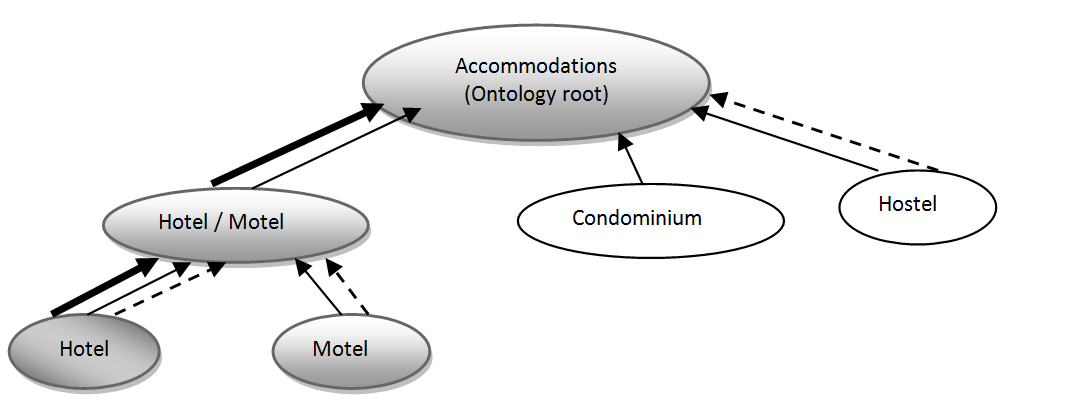
\includegraphics[width=120mm]{algorithm1.png}
\caption{Graphical representation of an Ontology}
\label{fig:graphonto}
\end{figure}

Figure \ref{fig:graphonto} illustrates the calculation of class divergence. This sample ontology is rooted at the class \textit{Accommodations}. The arrows represent the inheritance relationship between the classes in the topology.
Suppose we want to find the divergence $d_{class}(Hotel,Motel)$. Both are subclasses of the class \textit{Hotel/Motel} ($C$). They share the path from \textit{Hotel/Motel} to the $root$. So, the unnormalized divergence $d(Hotel, root)$ is two (shown by bold arrows), $d(Motel, Hotel/Motel)$ is one (dashed arrow), and $d(Hotel, Hotel/Motel)$ is one (dashed arrow). Thus, $d(Hotel, Motel)$ is four, which corresponds to a normalized value of $2/3$. 
Consider $d_{class}(Motel,Hostel)$. The classes $root$ and $C$ in the definition of $d_{class}$ are the same in this case so we add $d(Motel,Accommodations)$ (two), $d(Hostel, Accommodations)$ (one), and $d(Motel,Accommodations)$ (two), yielding a total unnormalized divergence of five, or a normalized divergence of $5/6$.


%-------------------------------------------------------------------------------

\subsection{QRM Ontology Matching}
\label{sec:oqom}

We use class divergence to calculate the relevance between a source SSQ and a target SSQ associated with a QRM.  Each SSQ will have four input classes, four output classes, and one realm.  We refer to the sequence of these classes $\langle \Upsilon_1, ..., \Upsilon_4, \Omega_1, ..., \Omega_4, R \rangle$ as the signature of an SSQ. If an input or output class is unspecified in the query, it is associated with the class $bottom$, which has no subclasses or individuals.

The relevance of QRM $Q$ with signature $\langle \Upsilon_{Q_1}, ..., \Upsilon_{Q_4}, \Omega_{Q_1}, ... , \Omega_{Q_4}, R_Q \rangle$ to SSQ $S$ with signature $\langle \Upsilon_{S_1}, ..., \Upsilon_{S_4}, \Omega_{S_1}, ... , \Omega_{S_4}, R_S \rangle$ is

\begin{equation}
\label{qrmsimilarity}
R\left({S,Q}\right) = 1- \pi_9 d_{class}(R_S,R_Q) + \sum_{k=1}^4\pi_k d_{class}(\Upsilon_{S_k},\Upsilon_{Q_k})+ \sum_{j=1}^4\pi_{4+j}d_{class}(\Omega_{S_j},\Omega_{Q_j})
\end{equation}

\noindent where the weights ${\pi}_k$ of the property hasRealm and other context properties satisfies the conditions 
\begin{equation}
\label{piconstraint1}
\sum_{k=1}^{9} {{\pi}_k} = 1
\end{equation}
\noindent and for $1 \leq i \leq 9$
\begin{equation}
\label{piconstraint2}
{\pi}_i > 0
\end{equation}

If an SSQ and a QRM have identical classes for all inputs, all outputs, and their realms then the QRM relevance value will be one. Otherwise, the relevance of the QRM will be in the range $[0, 1)$.   

%-------------------------------------------------------------------------------

\subsection{Ontological Structural Similarity}
\label{sec:oss}
Employing user input brings about the likelihood that redundant ontological elements will be inserted into our context class ontology. The work described here is aimed at finding ontological similarities between our context classes and QRMs so that we can reduce the number of redundant and incomparable elements. The ontological structural measure is determined by examining the ontological structure and semantics of each QRM. Our analysis depends on the ontology entities such as classes, individuals, properties, superclasses, and subclasses. The structural similarity is obtained from the following dissimilarity measures. 
 
\textit{\textbf{(a)}} class dissimilarity: This measure ($dist_{class}$) is determined by these features of the source and target classes: class URIs, parent classes, and class properties. 

\textit{\textbf{(b)}} property dissimilarity: This measure ($dist_{property}$) is determined by these features of the source and target class properties: property URIs, property domains ($classes$), and property ranges ($classes$). 

\textit{\textbf{(c)}} individual dissimilarity: This measure ($dist_{individual}$) for the source and target individuals is determined by their URIs, properties, and class types.

\subsubsection{Class dissimilarity}
Let $S$ be a source class and $T$ be a target class. The set of all the parent classes of the class $C$ is $parent(C)$ and the set of all the properties of the class $C$ is $property(C)$. We define two levels of class dissimilarity.\\
\indent \textit{\textbf{Level 0:}} In this level, the distance is measured using the dissimilarity between the OWL entity URIs ($dist_{URI}$):

\begin{enumerate}

\item URI dissimilarity for source and target classes 
\\ $f_1(S, T) = dist_{URI}(S.{uri},T.{uri})$  

\item URI dissimilarity for all the class properties
\\$f_2(S, T) = dist_{URI}(property_i.{uri},property_j.{uri}), 
\\\forall property_i \in property(S),\quad\forall property_j \in property(T) $

\item URI dissimilarity for all the parent classes
\\$f_3(S, T) = dist_{URI}(class_i.{uri},class_j.{uri}), 
\\\forall class_i \in parent(S),\quad \forall class_j \in parent(T) $

\end{enumerate}

\indent \textit{\textbf{Level 1:}} Here we calculate the URI dissimilarity in the same manner as in Level 0. It calculates class dissimilarity [Eq. \eqref{classsimilarity}] and property dissimilarity [Eq. \eqref{propertysimilarity} ] for each parent classes and the properties of the source and target classes.  The two additional steps are:
\begin{enumerate}

\item Compute property dissimilarity for all of the class properties 
\\$f_4(S, T) = dist_{property}(property_i,property_j), 
\\ \forall property_i \in property(S),\quad \forall property_j \in property(T) $ 

\item Compute class dissimilarity for all of the super classes of the class 
\\$f_5(S, T) = dist_{class}(class_i,class_j),
\\\forall class_i \in parent(S),\quad\forall class_j \in parent(T) $

\end{enumerate}

\indent Finally, we combine all these distances into a combinatorial measure for the complete OWL class dissimilarity measure

\begin{equation}
\label{classsimilarity}
dist_{class}(S, T)= \sum_{i=1}^N {{\alpha}_i f_i(s, t)}
\end{equation}
\noindent where ${\alpha}_i$ is the weight for a feature $i$, $N$ is the number of features, and satisfies the conditions
\begin{equation}
\label{alphaconstraint1}
\sum_{i=1}^{N} {{\alpha}_i} = 1
\end{equation}
\noindent and 
\begin{equation}
\label{alphaconstraint2}
{\alpha}_i \geq 0  
\end{equation}


\subsubsection{Property dissimilarity}
Let $S_P$ be a source property and $T_P$ be a target property. The set of all the domain classes of the OWL property $P$ is $domain(P)$ and the set of all the range classes of the OWL property $P$ is $range(P)$. We define two levels of property dissimilarity.\\
\indent\textit{\textbf{Level 0:}} In this level, the distance is measured using the dissimilarity between the OWL entity URIs ($dist_{URI}$):
\begin{enumerate}
    \item URI dissimilarity for source and target properties 
    \\ $f_1(S_P, T_P)= dist_{URI}(S_P.{uri}, T_P.{uri})$

    \item URI dissimilarity for source and target property domains
    \\ $f_2(S_P, T_P)= dist_{URI}(class_i, class_j ), 
    \\ \forall class_i \in domain(S_P),\quad\forall class_j \in domain(T_P)$

    \item URI dissimilarity for source and target property ranges
    \\ $f_3(S_P, T_P)= dist_{URI}(class_i, class_j ),
    \\ \forall class_i \in range(S_P),\quad\forall class_j \in range(T_P)$
\end{enumerate}

\indent\textit{\textbf{Level 1:}} Here we calculate the URI dissimilarity for domain and ranges of both the  source and target properties, in the same manner as in Level 0. Additionally, we calculate class dissimilarity [Eq. \eqref{classsimilarity}] for both domain and range. The two additional steps are:
\begin{enumerate}
    \item Compute property domain dissimilarity for all domains 
    \\ $f_4((S_P, T_P)= dist_{class}(class_i, class_j ),
    \\ \forall class_i \in domain(S_P),\quad \forall class_j \in domain(T_P)$

    \item Compute property range dissimilarity for all ranges  
    \\ $f_5(S_P, T_P)= dist_{class}(class_i, class_j),
    \\\forall class_i \in range(S_P),\quad \forall class_j \in range(T_P)$
\end{enumerate}
\indent Finally, we combine all these distances into a combinatorial measure for the complete OWL property dissimilarity measure
\begin{equation}
\label{propertysimilarity}
dist_{property}(S_P, T_P) = \sum_{i=1}^N {{\beta}_i f_i(S_P, T_P)} 
\end{equation}
where ${\beta}_i$ is the weight for a feature $i$ and satisfies the conditions 
\begin{equation}
\label{betaconstraint1}
\sum_{i=1} {{\beta}_i} = 1
\end{equation}
and 
\begin{equation}
\label{betaconstraint2}
{\beta}_i \geq 0
\end{equation} 


% --------------------------------------------------------------------------------

\section*{Future Work}
The QRMS are generalized representations of actual user queries. We are currently building the application engine that executes QRMs which are matched to a user query. Additionaly, we are working on leveraging our matching algorithm to chain multiple QRMs to create new web interactions.

We are building a statisical translation model to take natural language questions and turn them in to SSQs. We have begun a user study to identify how users can naturally translate their queries into our SSQ model. We anticipate that the user will not need to define the SSQ in the future but the translation will be automatic.

The current implementation does not consider \textit{modifiers} in finding the dissimilariy measure between context properties.  If the order of the \textit{modifiers} is changed within a context class, there could be an impact on the meaning of a query.  We will incorporate this consideration into our matching algorithms.

In addition, another step is to consider \textit{online execution} as a class similarity matching problem.  We can then build classifier systems using the machine learning techniques. Similarly, we can extend the QRM merging process during \textit{offline execution} to a clustering problem and implement conventional statistical methods to solve it. Finally, the parameters $\alpha$, $\beta$, and $\pi$ mentioned in the equations [Eq. \eqref{classsimilarity}, \eqref{propertysimilarity}, and \eqref{qrmsimilarity}] are defined manually. We are considering estimation methods that will be able to capture the relevance of the contexts, realm, and modifers of the QRM ontologies.     

% --------------------------------------------------------------------------------


\section*{Conclusion}
We have developed ontologies to model user web interaction and user web queries. We have also presented a matching algorithm to discover user web interactions based on a query. Our descriptions are in the OWL language. While we develop our own classes, because of the unified language, our class structure works well with existing ontologies such as \emph{dbpedia} and the \emph{New York Times} corpus. This model will allow question answering systems to use the deep web as a corpus.

% --------------------------------------------------------------------------------


\bibliography{citations}
\bibliographystyle{acm}

\end{document}
